%%
%% Beuth Hochschule für Technik --  
%%
%% Kapitel 5 - 
%%
%%	

\newpage

[Perkowski]
\section{Simulation des Steuer- und Störverhaltens der Strecke} \label{Kapitel5}
Zur Überprüfung der Modellierung mit Simulink wird mit Stelleinrichtung, Strecke, Messeinrichtung sowie Erregungssignale, wie im Kapitel drei und vier gewählt wurden, durchgeführt. Das simulierte System wird in den Arbeitspunkt erregt, und dann zusätzlich mit der Störung zugeschaltet. So konnten wir das Verhalten der Strecke mit der Störung analysieren.

\begin{figure}[h]
	\begin{center}
		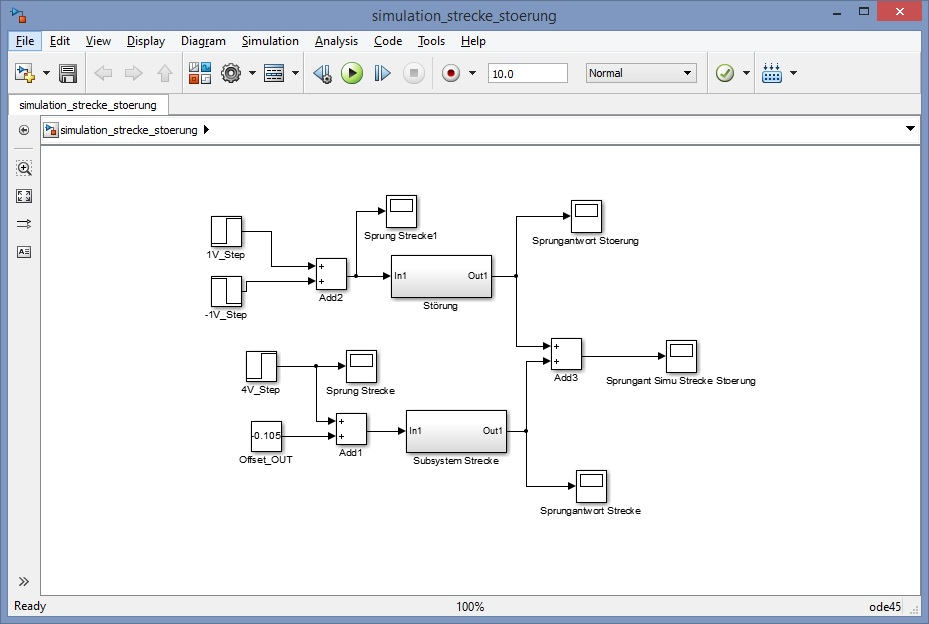
\includegraphics[scale=0.5]{simulink_simo_strecke_err.jpg}
		\caption{Simulink Simulationstrecke mit Störung}
       \label{simustreckestor}
	\end{center} 
\end{figure}

\begin{figure}[h]
	\begin{center}
		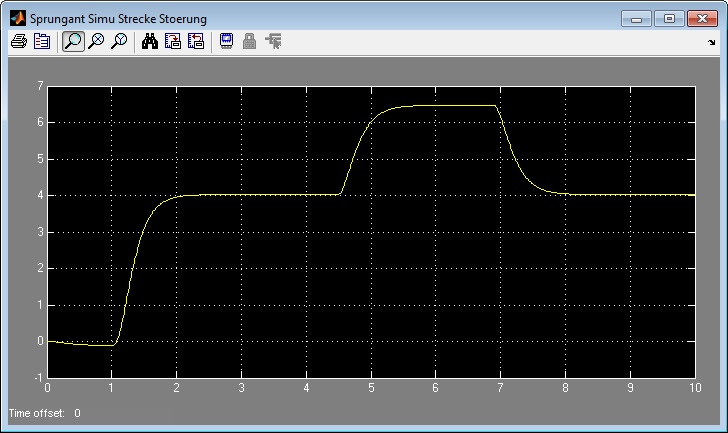
\includegraphics[scale=0.5]{simu_strecke_stoerung.jpg}
		\caption{Systemantwort Simulationstrecke mit Störung}
       \label{plotsimustreckestor}
	\end{center} 
\end{figure}

